\documentclass[Bachelorarbeit.tex]{subfiles}
\begin{document}

\graphicspath{{./figures/interpretation/}}	%specifying the folder for the figures

\chapter{Interpretation}
\label{ch:interpretation}

In this chapter the interpretation of the results of chapter \ref{ch:results} are given and discussed where the central question is whether the hypothesis is sufficient that is if Ascending-Connected topology reaches the theoretical equilibrium. Thus only this topology is handled - both with and without importance sampling - because it is the most minimal network which satisfies the requirements for the hypothesis. The interpretations for the results of hub-, scale-free and small-world topologies are handled in appendix \ref{app:results} but only to a minimal extent as they turn out to fall far from satisfying the hypothesis and the theoretical equilibrium because almost all of them do not meet the requirements but show interesting behaviour.

\section{Validating the Hypothesis}
When comparing the results of Ascending-Connected topology of figure \ref{fig:wealth_ASCENDINGCONNECTED_100_NOCOLLATERALMARKET_REPL} with the results of the Fully-Connected topology of figure \ref{fig:wealth_FULLYCONNECTED_100_NOCOLLATERALMARKET_REPL} it becomes immediately clear that the equilibrium is different from the one of the Fully-Connected network and thus theoretical equilibrium is not reached in the case of Ascending-Connected without importance sampling. Although the visual results come quite close to the Fully-Connected one where there is a clear distinction between pessimists, medianists and optimists there remain serious artefacts in the wealth-distribution. Thus the hypothesis is invalid as the property postulated is just necessary but not sufficient to reach theoretical equilibrium. 

\section{Analysing artefacts}
Obviously the artefacts in the range of the pessimists and medianists and partly of the optimists indicate a miss-allocation of wealth. Pessimists, as noted in chapter \ref{ch:leverageCycle} are maximally short on assets and bonds and hold only cash but the results violate this prediction as the pessimists still hold free- and collateralised assets and a few bonds. Medianists should hold only bonds but have still cash and free assets left and the optimists have still a big chunk of free assets left. As will be shown it comes from the fact that the pessimists want to sell but no neighbour is able to buy any more - a scenario which is not possible in Fully-Connected topology and is thus unique to Ascending-Connected networks with and without importance sampling. In fully-connected networks all agents are connected with each other thus if there is any agent who wants to sell some good there will be statistically speaking not only 1 potential buyer as in ascending-connected networks but a much larger range, depending on the sellers optimism-factor and the number of agents. In ascending-connected networks each seller has only one buyer where this buyer is at the same time the seller for the next buyer and so on. This can lead to situations where one seller wants to sell goods but its buyer can't buy any more as it has already sold e.g. all assets in its role as seller and is thus unable to satisfy the sellers offer due to trading constraints. Even worse a buyer farther away could satisfy the sell-offer but is not directly connected to the seller so they can't trade although both would potentially match.

\subsection{Dynamics of a single run}
\label{sub:dynamics_singlerun}
To better understand how such artefacts arise one needs to investigate the dynamics of a single run of the Ascending-Connected topology. The tools used are both the \textit{market-activity} and \textit{wealth-distribution} diagrams where the former one shows for each point of time the relative activity strength of each market. Being active means a successful match on a given market which implies that in a successful matching-round only one market can be active as only one match on a specific market happens during a successful matching round. Because of this a moving window of size 100 is used to create a moving-average filter over all active markets where the result is normalized and all market-activity sums to 1.0 at each point in time of the diagram. This allows for a very good visual analysis of distinct trading-stages because noise is reduced but the overall trend of a market can be still seen clearly.

\medskip

\begin{figure}[H]
	\centering
  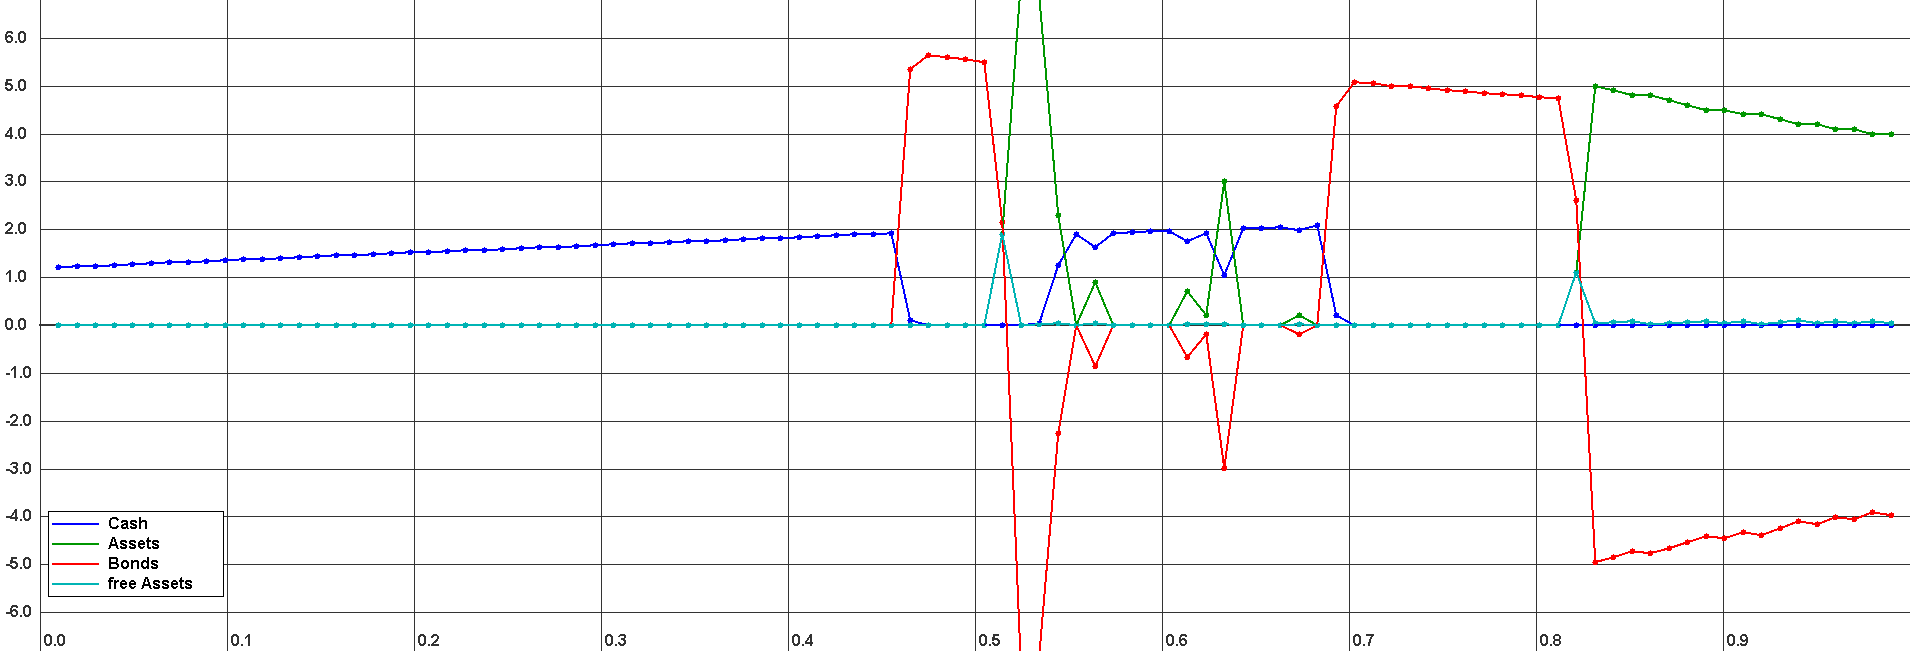
\includegraphics[width=1.0\textwidth, angle=0]{ASCENDINGCONNECTED_100_NOCOLLATERALMARKET_SINGLE.png}
	\caption{Final wealth-distribution after a single run of the Ascending-Connected topology. Note the artefacts in the range of the pessimists. The following wealth-distributions are all taken from various points in time of this single run.}
	\label{fig:wealth_ASCENDINGCONNECTED_100_NOCOLLATERALMARKET_SINGLE}
\end{figure}

\begin{figure}[H]
	\centering
  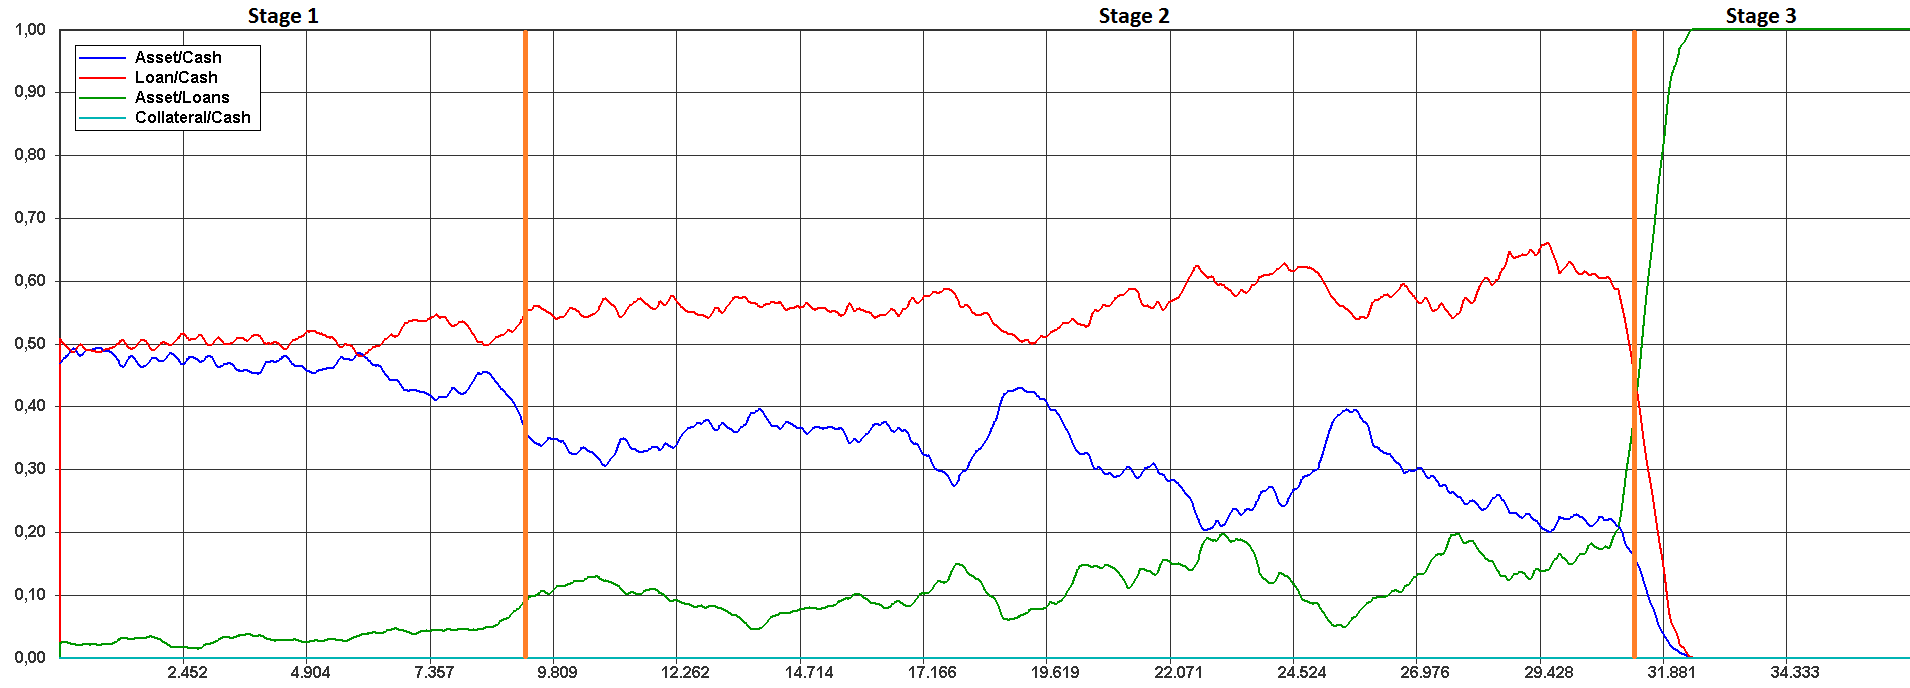
\includegraphics[width=1.0\textwidth, angle=0]{ASCENDINGCONNECTED_100_NOCOLLATERALMARKET_MARKET_STAGES.png}
  	\caption{Market-activity stages of the single run of figure \ref{fig:wealth_ASCENDINGCONNECTED_100_NOCOLLATERALMARKET_SINGLE}}
	\label{fig:markets_ASCENDINGCONNECTED_100_NOCOLLATERALMARKET_MARKET_STAGES}
\end{figure}

3 trading-stages can be identified in the market-activity diagram \ref{fig:markets_ASCENDINGCONNECTED_100_NOCOLLATERALMARKET_MARKET_STAGES}.

\paragraph{Stage 1}
The allocations are very random overall but pessimists are already emerging which can be seen at the very left end of the wealth-range. They sell their free assets against cash thus holding primarily cash. The optimists are beginning to emerge as well by buying as many assets they can which can be seen at the very right end of the wealth-range. The medianists are far from showing up.

\medskip

The Asset/Cash and Asset/Bond markets are very dominant in this stage as the pessimists try to get cash for their free assets and the optimists try to buy assets against cash and bond. The Bond/Cash market is not as active but nevertheless contributes as well because optimists using bonds to leverage their asset trades and pessimists try to get their bonds towards the optimists by using the BP-mechanism.

\begin{figure}[H]
	\centering
  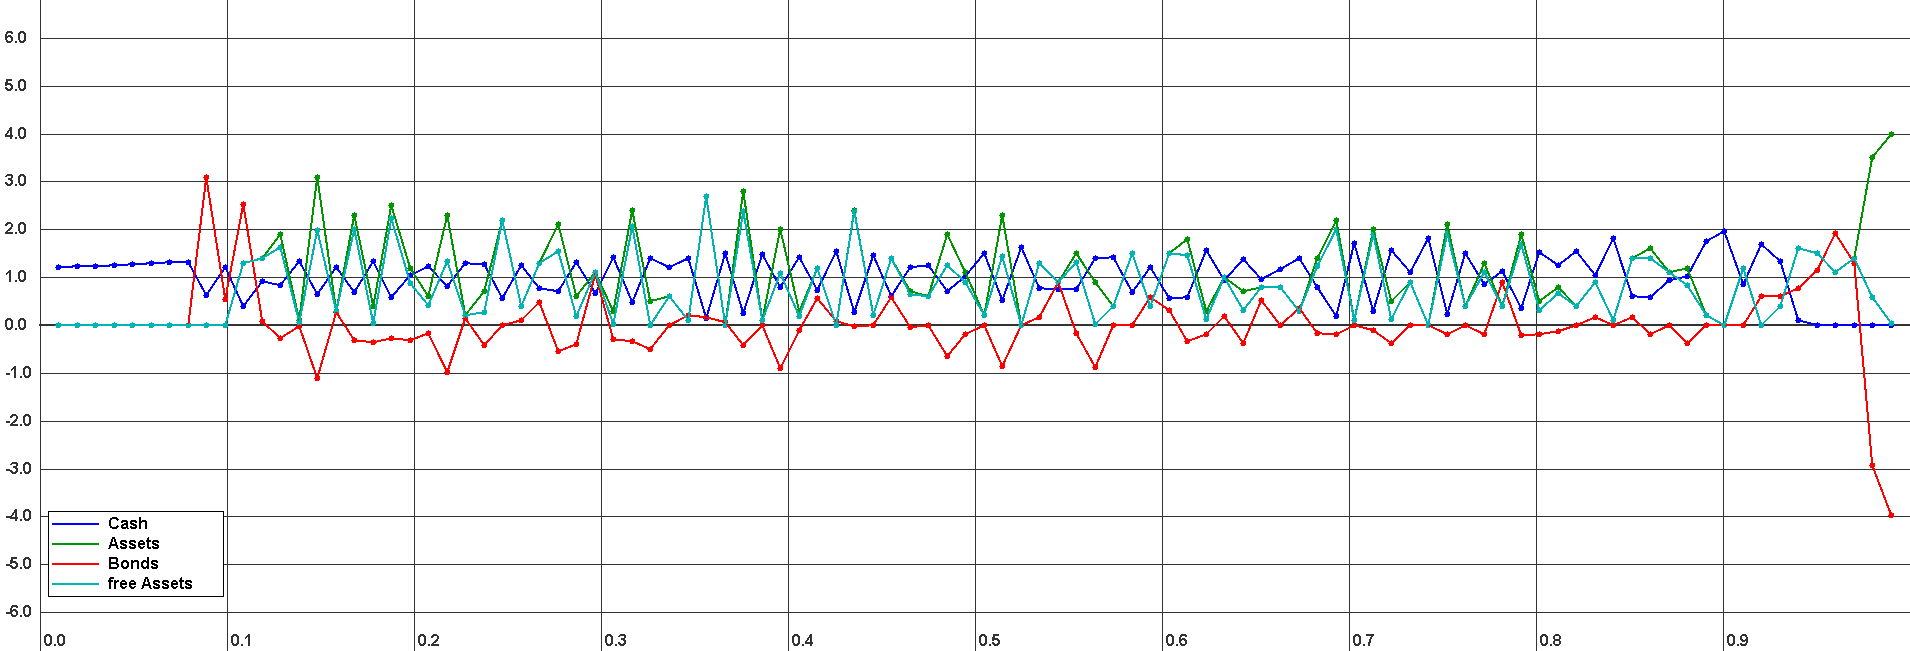
\includegraphics[width=1.0\textwidth, angle=0]{ASCENDINGCONNECTED_100_NOCOLLATERALMARKET_WEALTH_STAGE_1.png}
  	\caption{Wealth-Distribution of Ascending-Connected topology during Stage 1 of the single run of figure \ref{fig:wealth_ASCENDINGCONNECTED_100_NOCOLLATERALMARKET_SINGLE}.}
	\label{fig:markets_ASCENDINGCONNECTED_100_NOCOLLATERALMARKET_WEALTH_STAGE_1}
\end{figure}

\paragraph{Stage 2}
The pessimists are clearly visible and hold both bonds and collateralized assets which they try to trade up to the optimists. The optimists are also clearly visible as  they are maximally short on cash and hold either free or collateralized assets. The medianists are still not visible yet.

\medskip

The Asset/Cash market seems to go down in the long term while the Bond/Cash and Asset/Bond markets seems to increase. This is because fewer and fewer assets can be traded against cash because the optimists are already very low on cash thus the Asset/Bond market is naturally increasing as they can trade only on this market any more.

\begin{figure}[H]
	\centering
  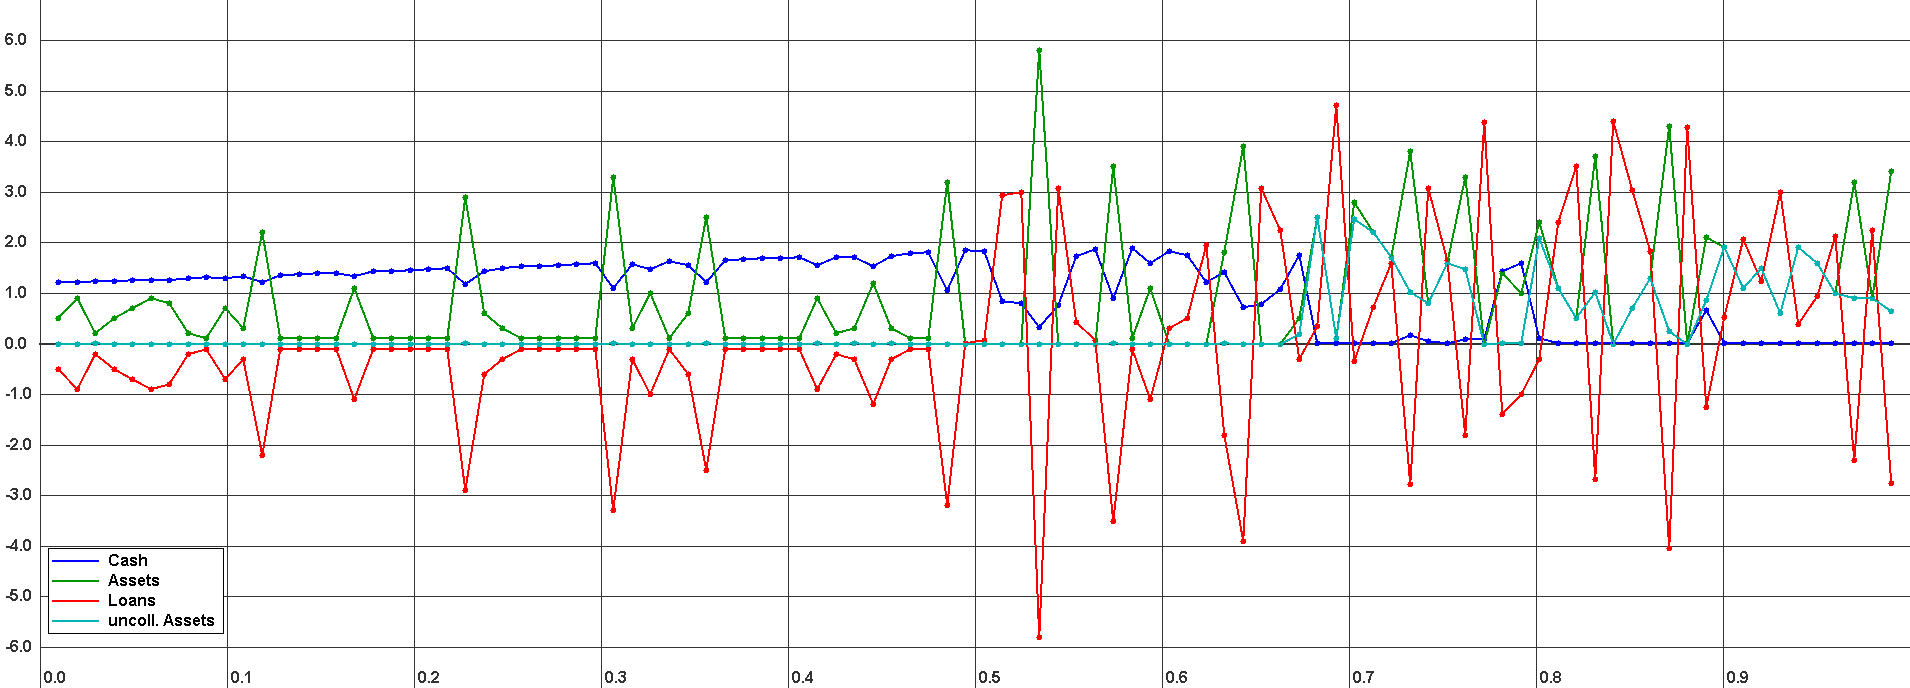
\includegraphics[width=1.0\textwidth, angle=0]{ASCENDINGCONNECTED_100_NOCOLLATERALMARKET_WEALTH_STAGE_2.png}
  	\caption{Wealth-Distribution of Ascending-Connected topology during Stage 2 of the single run of figure \ref{fig:wealth_ASCENDINGCONNECTED_100_NOCOLLATERALMARKET_SINGLE}.}
	\label{fig:markets_ASCENDINGCONNECTED_100_NOCOLLATERALMARKET_WEALTH_STAGE_2}
\end{figure}
		
\paragraph{Stage 3}
The pessimists lie dormant and are completely inactive. Although they still hold positive bonds and free- and collateralized assets they have become unable to trade them towards the optimists. The reason for this is investigated in the next section. The medianists begin to show up holding only bonds and free- and collateralized assets. The optimists try to get their hands on these free- and collateralized assets which they can only do by trading assets for bonds because they have no more cash. Thus these two frontiers move towards each other and will result in the final wealth-distribution found in figure \ref{fig:wealth_ASCENDINGCONNECTED_100_NOCOLLATERALMARKET_SINGLE}.

\medskip

The Asset/Cash and Bond/Cash markets decline completely because the pessimists are no more able to trade as outlined above and the optimists and medianists are maximally low on cash thus being unable to make offers on these markets too. The Asset/Bond market takes over and dominates 100\% as the medianists hold only free- and collateralized assets any more which the optimists want to buy which they can only do through this market by taking a bond for buying the asset.

\begin{figure}[H]
	\centering
  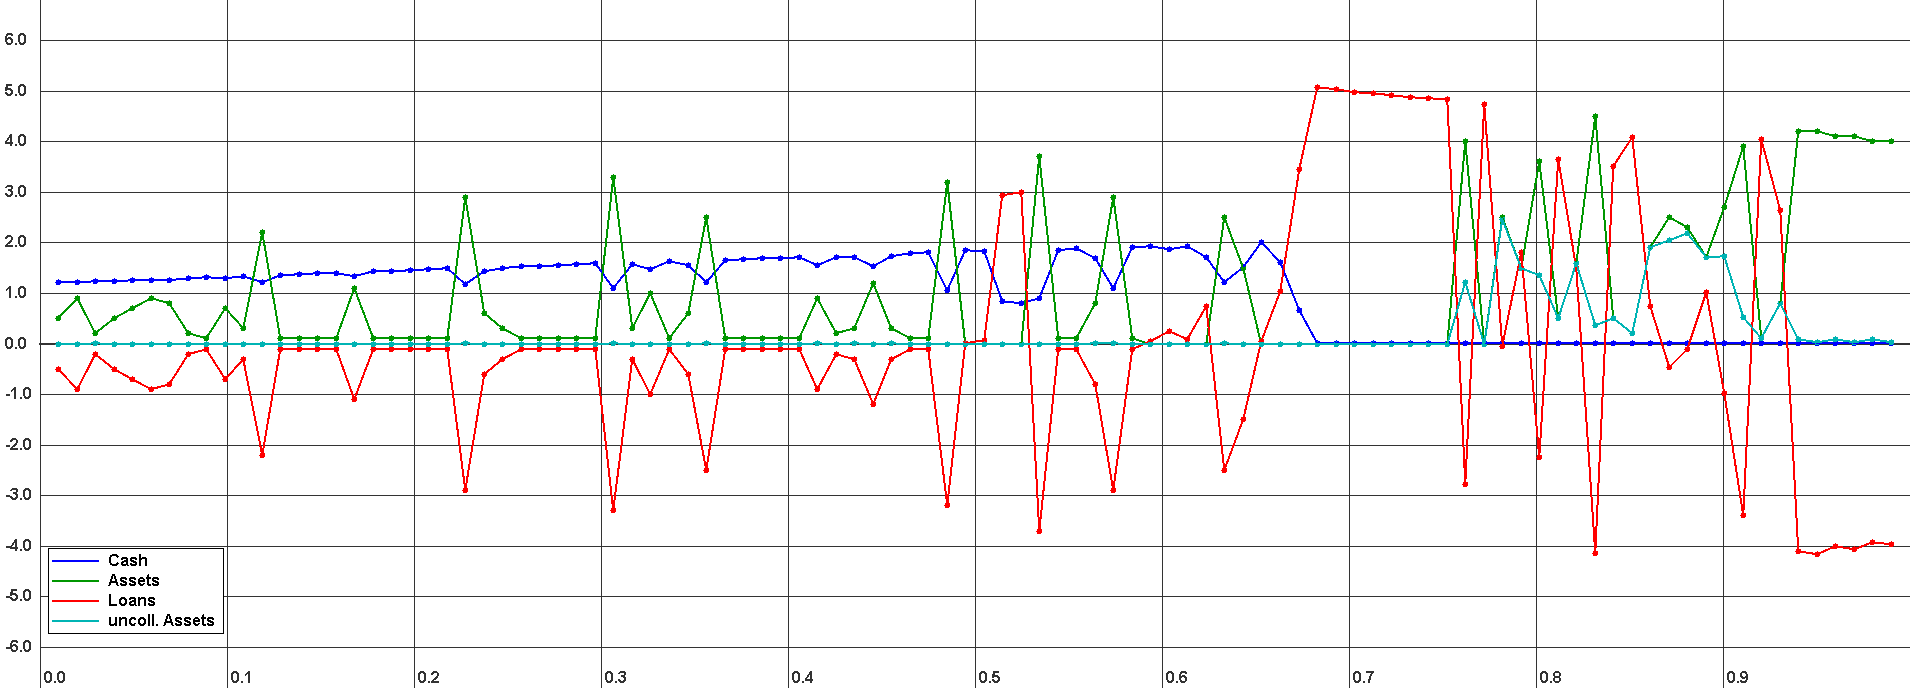
\includegraphics[width=1.0\textwidth, angle=0]{ASCENDINGCONNECTED_100_NOCOLLATERALMARKET_WEALTH_STAGE_3.png}
  	\caption{Wealth-Distribution of Ascending-Connected topology during Stage 3 of the single run of figure \ref{fig:wealth_ASCENDINGCONNECTED_100_NOCOLLATERALMARKET_SINGLE}.}
	\label{fig:markets_ASCENDINGCONNECTED_100_NOCOLLATERALMARKET_WEALTH_STAGE_3}
\end{figure}

\section{Deriving the emerging of the artefacts}

\subsection{Blocking-Situation prevents trading} As already outlined the artefacts arise due to a blocking situation where trading becomes and \textit{stays} impossible between two neighbours. The seller places ask-offerings on a given market but due to trading constraints the only potential buyer which is the neighbour with the next higher optimism-factor can't place any potential matching bid-offering on the given market. In figure \ref{fig:wealth_ASCENDINGCONNECTED_100_NOCOLLATERALMARKET_SINGLE} this blocking-situation can be seen between the agent-pairs 55 (0.545) \& 56 (0.554), 57 (0.564) \& 58 (0.574), 62 (0.614) \& 63 (0.624), 64 (0.634) \& 65 (0.644) and 68 (0.673) \& 69 (0.683). In all pairs the seller, which is the agent with the lower optimism-factor, holds only collateralized assets and thus places ask-offers only on the Asset/Bond market. The buyer, which is the agent with the higher optimism-factor, holds only cash and places bid-offers only on the Asset/Cash and Bond/Cash market but not on the Asset/Bond market - trading has become impossible between the two agents. It is interesting to see that the wealth-distribution in the range of 0.455 - 0.554 already shows basic similarities to the global distribution because all wealth is traded up towards the blocking-point creating the small sub-distribution of pessimists, medianists and optimists.

\subsection{Situation can occur only on the Asset/Bond market.} An agent can hold a mix of cash, free assets and positive bonds or collateralized assets. To show that the situation can occur only on the Asset/Bond market one must investigate the combinations of allocations and possible trading options.

\begin{enumerate}
\item Seller has cash, buyer any goods \\ Seller does not sell anything. 
\item Seller has positive bonds, buyer has cash \\ Buyer can buy from seller through the BP-mechanism.
\item Seller has positive bonds, buyer has free assets \\ No direct trading with these goods but buyer will act as seller and can sell assets up to optimists on Asset/Cash market thus generating cash which creates then the same situation as in 2.
\item Seller has positive bonds, buyer has collateralized assets \\ No trading with these goods but buyer will act as seller towards higher optimists on the Asset/Bond market thus creating uncollateralized assets and thus creating cash thus enabling to buy the positive bonds which creates then the same situation as in 2.
\item Seller has free assets, buyer has cash \\ Buyer can buy assets from seller against cash.
\item Seller free assets, buyer has positive bonds \\ Buyer can by the assets against bonds.
\item Seller has free assets, buyer has collateralized assets \\ Buyer can buy free assets against bonds.
\item Seller has collateralized assets, buyer has positive bonds \\ Buyer can buy assets against bonds.
\item Seller has collateralized assets, buyer has free assets \\ No trading with these goods but buyer will act as seller and will sell assets up to optimists against cash or bonds, thus generating cash or positive bonds which is then same as in 8 or 10.
\item Seller: collateralized assets, buyer has cash \\ No trading with these goods as the buyer has no possibility to buy the collateralized assets against cash. In the role of a seller it can't sell anything to transform cash to other goods which could potentially unlock this situation.
\end{enumerate}

The critical situation is the one given in the last point. As long as an agent has a mix of goods allocated then the blocking situation does not occur as trading is possible through a different channel than the last one. However if the allocations result in an extreme where the seller holds \textit{only} collateralized assets and the buyer \textit{only} cash then the blocking-situation occurs and is impossible to unlock any more.

\subsection{Artefacts are random} An important fact to notice is that the artefacts must not necessarily show up. It is possible for a single run to finish without these artefacts showing up. This is due to the random-process of sweeping and matching and thus the artefacts are subject to this random process too as noted in section \ref{sec:implementation_performanceImprovement}. When looking at the result of Ascending-Connected topology with importance sampling in figure \ref{fig:wealth_ASCENDINGCONNECTED_IS_100_NOCOLLATERALMARKET_REPL} it seems that Importance sampling elevates this problem as no artefacts have shown up during an experiment with 50 replications. This however is no proof that importance sampling is the solution to this problem as the mechanism is still the same. We conjecture that due to the dramatically increased matching-probabilities the occurrence of such miss-allocations have become highly unlikely but are not guaranteed to never show up any more thus the importance sampling is not accepted as a remedy for the miss-allocations. In a special experiment with 200 replications artefacts have shown up which proofs that importance sampling is definitely not a remedy for the miss-allocations.

\subsection{Formal proof using utility-functions}
It is of very importance to note that an agent can never have a total utility of 0 in this simulation. Per definition in chapter \ref{ch:leverageCycle} each trade results in an increase of the utility. If the agents start with the basic endowment of 1 unit of cash and 1 unit of assets as given in chapter \ref{ch:leverageCycle} then they will start already with a utility $\geq 0$. Thus it can never reach 0.

\medskip

TODO: einleitende worte, wieso über utility-function

\begin{align*}
	utility = u_{asset} + u_{bond} + u_{cash}
	\\ = limit_{asset} \; holdings_{asset} + \\
			limit_{bonds} \; holdings_{bonds} + \\
			(sell_{asset} - buy_{asset}) \; price_{asset} + \\
			(give_{bonds} - take_{bonds}) \; price_{bonds} + \\
			holdings_{cash} 
\end{align*}

Substituting allocations of seller with only collateralized assets and buyer with only cash to get the utility \textit{before} the potential trade.

\begin{align*}
	utility_{seller} = limit_{asset} \; holdings_{asset} - \\
			limit_{bond} \; holdings_{bond} \\
\end{align*}

Note that $holdings_{asset} = holdings_{bond}$ because all assets are collateralized and thus for all taken bonds the equal amount of assets is held as security.

\begin{align*}
	utility_{buyer} = holdings_{cash} 
\end{align*}

Regarding the utility-functions the following trades are theoretically possible:
\begin{itemize}
\item Buyer buys the assets only and leaves the bonds to the seller.
\item Buyer buys the negative bonds only and leaves the assets to the seller.
\item Buyer buys both the assets and the negative bonds from the seller. possibility would be to trade both the assets and the bonds, which amounts to trading collateralized assets, but that market exists not.
\end{itemize}

Now each possibility is investigated in regard to the utility-functions and we demand as defined in chapter \ref{ch:leverageCycle} that each trade results in a utility-gain thus $utiliy_{after} > utility_{before}$ must hold.

\paragraph{Buyer buys all the assets only for cash and leaves the bonds to the seller.}
The utilities \textit{after} the trade are

\begin{align*}
	utility_{buyer} = limit_{asset} \; holdings_{asset} - \\
				buy_{asset} \; price_{asset} + \\
				holdings_{cash}
\end{align*}

\begin{proof}
\begin{align*}
	utiliy_{after} > utility_{before} 
		\\ = limit_{asset} \; holdings_{asset} - \\
			buy_{asset} \; price_{asset} + \\
			holdings_{cash} > holdings_{cash}		\tag*{$| -holdings_{cash}$}
		\\ = limit_{asset} \; holdings_{asset} - \\
			buy_{asset} \; price_{asset} > 0		\tag*{$| holdings_{asset} = buy_{asset}$}
		\\ = limit_{asset} \; buy_{asset} - \\
			buy_{asset} \; price_{asset} > 0		\tag*{$|:buy_{asset}$}
		\\ = limit_{asset} - price_{asset} > 0
		\\ = limit_{asset} > price_{asset}			
\end{align*}
\end{proof}

\begin{align*}
	utility_{seller} = -limit_{bond} \; holdings_{bond} + \\
				sell_{asset} \; price_{asset}
\end{align*}

\begin{proof}
\begin{align*}
	utiliy_{after} > utility_{before} 
		\\ = -limit_{bond} \; holdings_{bond} + \\
				sell_{asset} \; price_{asset} > \\
				limit_{asset} \; holdings_{asset} - \\
				limit_{bond} \; holdings_{bond} 		
		\\ = sell_{asset} \; price_{asset} > \\
				limit_{asset} \; holdings_{asset}		\tag*{$| sell_{bond} = holdings_{asset}$}
		\\ = sell_{asset} \; price_{asset} > \\
				limit_{asset} \; sell_{asset}			\tag*{$|:sell_{asset}$}
		\\ =  price_{asset} > limit_{asset}		
		\\ =  limit_{asset}	< price_{asset}	
\end{align*}
\end{proof}
	
Thus it is proven that $limit_{buyer} > price_{asset} > limit_{seller}$ which is only possible if the buyer has a higher optimism-factor than the seller which was already proven in chapter \ref{ch:hypothesis}. Unfortunately this trade is not allowed as it would violate the collateral constraint which enforces that for each taken bond the same amount of assets must be hold as security. 

\paragraph{Buyer buys the negative bonds only and leaves the assets to the seller.}
The utilities \textit{after} the trade are

\begin{align*}
	utility_{buyer} = -limit_{bond} \; holdings_{bond} - \\
				buy_{bond} \; price_{bond} + \\
				holdings_{cash}
\end{align*}

\begin{proof}
\begin{align*}
	utiliy_{after} > utility_{before} 
		\\ = -limit_{bond} \; holdings_{bond} - \\
				buy_{bond} \; price_{bond} + \\
				holdings_{cash} > holdings_{cash}		\tag*{$| -holdings_{cash}$}
		\\ = -limit_{bond} \; holdings_{bond} - \\
				buy_{bond} \; price_{bond} > 0			\tag*{$| \; holdings_{bond} = buy_{bond}$}
		\\ = -limit_{bond} \; buy_{bond} - \\
			buy_{bond} \; price_{bond} > 0				\tag*{$|:buy_{bond}$}
		\\ = -limit_{bond} - price_{bond} > 0			\tag*{infeasible as limit-price and price are $> 0$}
\end{align*}
\end{proof}

The utility-gain for the buyer is impossible in this trade thus it is rejected.

\paragraph{Buyer buys both the assets and the negative bonds from the seller.}
\begin{align*}
	utility_{buyer} = limit_{asset} \; holdings_{asset} - \\
				limit_{bond} \; holdings_{bond} - \\
				buy_{asset} \; price_{asset} - \\
				buy_{bond} \; price_{bond} + \\
				holdings_{cash}
\end{align*}

\begin{proof}
\begin{align*}
	utiliy_{after} > utility_{before}
		\\ = limit_{asset} \; holdings_{asset} - \\
				limit_{bond} \; holdings_{bond} - \\
				buy_{asset} \; price_{asset} - \\
				buy_{bond} \; price_{bond} + \\
				holdings_{cash} > holdings_{cash}	\tag*{$| -holdings_{cash}$}
		\\ = limit_{asset} \; holdings_{asset} - \\
				limit_{bond} \; holdings_{bond} - \\
				buy_{asset} \; price_{asset} - \\
				buy_{bond} \; price_{bond} > 0		\tag*{$|$ all holdings and buy are same = h}
		\\ = limit_{asset} \; h - \\
				limit_{bond} \; h - \\
				h \; price_{asset} - \\
				h \; price_{bond} > 0				\tag*{$|:h$}
		\\ = limit_{asset} - limit_{bond} - \\
				price_{asset} - price_{bond} > 0
\end{align*}
\end{proof}

This is feasible as in case of the buyer $limit_{asset} > price_{asset}$ and $limit_{bond} > price_{bond}$ because the buyers limit-price is always above the final price as proven in \ref{ch:hypothesis}. Further $limit_{asset} > limit_{bond}$ holds.

\begin{align*}
	utility_{seller} = sell_{asset} \; price_{asset} + \\
				sell_{bond} \; price_{bond}
\end{align*}

\begin{proof}
\begin{align*}
	utiliy_{after} > utility_{before}
		\\ = sell_{asset} \; price_{asset} + \\
				sell_{bond} \; price_{bond} >
				limit_{asset} \; holdings_{asset} -
				limit_{bond} \; holdings_{bond}		\tag*{$|$ all holdings and sell are same = h}
		\\ = h \; price_{asset} + \\
				h \; price_{bond} >
				limit_{asset} \; h -
				limit_{bond} \; h					\tag*{$|:h$}
		\\ =  price_{asset} + price_{bond} >
				limit_{asset} - limit_{bond} 
\end{align*}
\end{proof}

This is feasible as in case of seller $limit_{asset} < price_{asset}$ and $limit_{bond} < price_{bond}$ because the sellers limit-price is always below the final price as proven in \ref{ch:hypothesis}. Further $limit_{asset} > limit_{bond}$ holds. Unfortunately this trade is not possible as it amounts to trading collateralized assets where no market does exist for it.

\section{Extending the Hypothesis}
After it has become clear that the hypothesis is not sufficient the question arises what needs to be done to approach the theoretical equilibrium anyway. It is clear that a mechanism needs to be found which prevents or resolves the arising of the artefacts within wealth-distribution. Obviously two solutions are available.

\subsection{Approaching fully connectedness}
Increasing the connectedness of the topology allows more agents to trade between each other and thus the probability of resolving islands or artefacts of wealth miss-allocation is increased with the density of connectedness. The experiments of ascending-connected topology with short-cuts were designed to develop an understanding how the simulation behaves with increasing connectedness and also how the two types of  fully- and regular-connectedness influence the results. It seems that full short-cuts seem to help dramatically in reducing the miss-allocations where the number of full short-cuts seems to be dependent on the number of agents which this thesis leaves for further research. See section \ref{app:results_acShortCuts} for a short overview of the results and interpretation of short-cut based Ascending-Connected topologies.
\linebreak
Of course in real environments approaching fully connectedness is not always possible and thus only the other mechanism is left as an option to resolve the artefacts.

\subsection{Re-Enabling trading}
\label{ch:interpretation_reenablingTrading}
Another way to look at the arising of the artefacts is in identifying them as suboptimal trades. \cite{Breuer2015} were confronted with this circumstance when they introduced the Asset/Bond Market where they found that the equilibrium was fundamentally different from the theoretical one because agents were trapped in suboptimal trades and couldn't reverse their decisions made earlier. The trades where suboptimal because each agent assigns depending on its optimism factor a different bond-value to each asset. As a solution they introduced the "Bonds-Pledgeability" (BP) mechanism which allows to trade bonds in both ways instead of only gathering them and not being able to sell them - see chapter \ref{ch:leverageCycle} for a more in-depth discussion of the BP-Mechanism.

\medskip 

Thus if those artefacts are treated as suboptimal trades where decisions of the traders lead to a specific blocking-situation in the context of collateralized assets as described above one needs to introduce a new mechanism to allow to repair such blocking-situations. The only possibility without altering the network-topology is to re-enable the pessimists to trade their collateralized assets against cash as all pessimists hold cash and are thus able to buy and sell collateralized assets against cash. This new mechanism is expected to repair the miss-allocated wealth and to restore the validity of the previously disproved hypothesis.

\medskip 

See chapter \ref{ch:newMarket} for the implementation and results of this new mechanism.

\end{document}
